\chapter{Resultados}
\label{chapter:resultados}

\section{Análisis de componentes principales}
\label{resultados:pca}
\subsection{Conjunto de datos completo}

\paragraph{}
Para este caso, al ejecutar el \textit{PCA} con el conjunto de datos completo, este nos muestra tal y como podemos ver en la figura \ref{pcaOneResult}, que con solo 3 atributos, el modelo es capaz de explicar (predecir) el 95\% de las observaciones.

\paragraph{}
\begin{figure}[!htb]
  \centering
    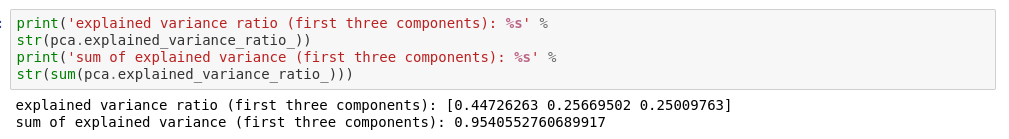
\includegraphics[width=0.9\textwidth]{images/resultados_procesado_de_datos_pca1_result.png}
    \caption{Resultado del \textit{PCA}.}
  \label{pcaOneResult}
\end{figure}

\paragraph{}
Dado que el \textit{PCA} solo nos muestra 3 atributos como relevantes, podemos representar los resultados de las observaciones a un gráfico que mostramos en la figura \ref{pcaOneGraphic} dibujando los 3 componentes principales como si fueran 3 dimensiones, y pintamos los valores a predecir sobre estos (aplicando el color rojo a las observaciones que no consideran útiles, y azul a los que si se consideran útiles), podemos observar que la gran mayoría de los rojo se encuentran en el plano del componente principal 1 y dos, mientras que el azul esta mas repartidos en los dos planos.

\paragraph{}
\begin{figure}[!htb]
  \centering
    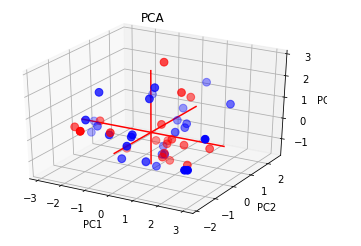
\includegraphics[width=0.3\textwidth]{images/resultados_procesado_de_datos_pca1_graphic.png}
    \caption{Proyección delos resultados del \textit{PCA} en una gráfica.}
  \label{pcaOneGraphic}
\end{figure}

\paragraph{}
Si le pedimos al modelo que nos indique cuales son los 3 componentes que ha detectado que son los principales, este nos muestra los resultados que se pueden ver en la figura \ref{pcaOneAtributos}. Para saber cuales son los componentes, tendremos que quedarnos para cada componente principal, el valor del atributo que más se acerque a 1.

\paragraph{}
\begin{figure}[!htb]
  \centering
    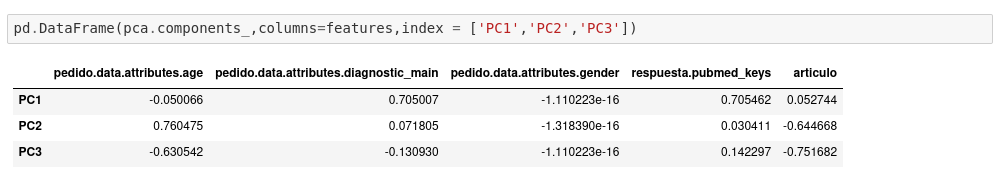
\includegraphics[width=0.9\textwidth]{images/resultados_procesado_de_datos_pca1_atributos.png}
    \caption{Proyección de los resultados del \textit{PCA} sobre los atributos del conjunto de datos.}
  \label{pcaOneAtributos}
\end{figure}

\paragraph{}
Para este caso, el \textit{PCA} nos muestra que los 3 componentes principales son, el atributo \textit{pubmed\_keys}, el atributo \textit{age} y el atributo \textit{diagnostic\_main}.

\subsection{Conjunto de datos solo con atributo utilidad definido}

\paragraph{}
En este caso, el \textit{PCA} nos muestra tal y como podemos ver en la figura \ref{pcaTwoResult}, que necesitamos 5 atributos para que el modelo sea capaz de explicar (predecir) el 97\% de las observaciones.

\paragraph{}
\begin{figure}[!htb]
  \centering
    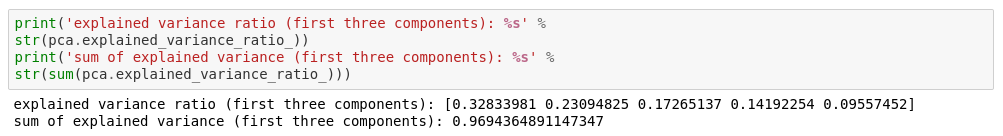
\includegraphics[width=0.9\textwidth]{images/resultados_procesado_de_datos_pca2_result.png}
    \caption{Resultado del \textit{PCA} de la segunda ejecución.}
  \label{pcaTwoResult}
\end{figure}

\paragraph{}
Para este caso, el \textit{PCA} nos muestra tal y como podemos ver en la figura \ref{pcaTwoAtributos}, que los 5 componentes principales son, el atributo \textit{diagnostic\_main}, el atributo \textit{Year}, el atributo \textit{pubmed\_keys}, el atributo \textit{age} y el atributo \textit{articulo}.

\paragraph{}
\begin{figure}[!htb]
  \centering
    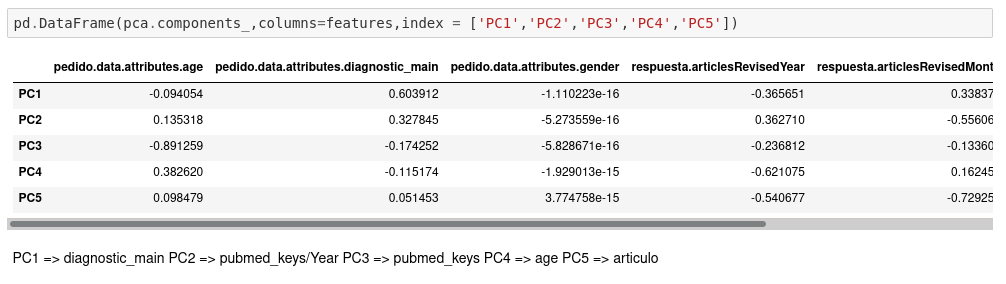
\includegraphics[width=0.9\textwidth]{images/resultados_procesado_de_datos_pca2_atributos.png}
    \caption{Proyección de los resultados del \textit{PCA} sobre los atributos del conjunto de datos para la segunda ejecución.}
  \label{pcaTwoAtributos}
\end{figure}

\subsection{Conjunto de datos solo con atributo utilidad definido, añadiendo el mes y año del articulo, eliminando los atributos \textit{gender} y articulo y expandiendo el atributo \textit{respuesta.pubmed\_keys}}

\paragraph{}
En este caso, el \textit{PCA} nos muestra tal y como podemos ver en la figura \ref{pcaThreeResult} , que necesitamos 4 atributos para que el modelo sea capaz de explicar (predecir) el 90\% de las observaciones.

\paragraph{}
\begin{figure}[!htb]
  \centering
    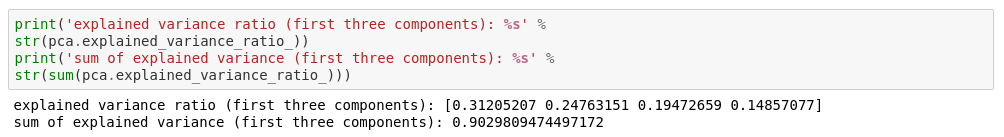
\includegraphics[width=0.9\textwidth]{images/resultados_procesado_de_datos_pca3_result.png}
    \caption{Resultado del \textit{PCA} de la tercera ejecución.}
  \label{pcaThreeResult}
\end{figure}

\paragraph{}
Para este caso, el \textit{PCA} nos muestra como podemos ver en la figura \ref{pcaThreeAtributos} , que los 4 componentes principales son, el atributo \textit{diagnostic\_main}, el atributo \textit{Month}, el atributo \textit{pubmed\_keys} y el atributo \textit{age}.

\paragraph{}
\begin{figure}[!htb]
  \centering
    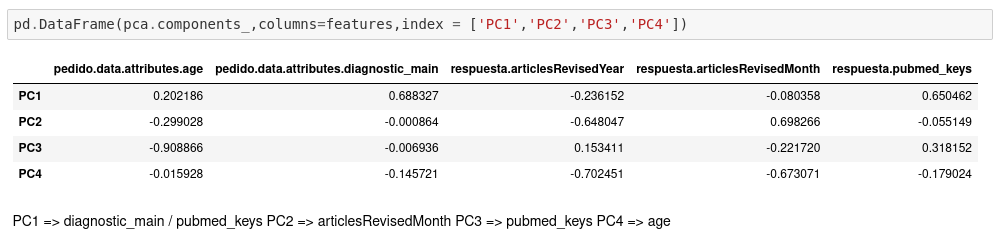
\includegraphics[width=0.9\textwidth]{images/resultados_procesado_de_datos_pca3_atributos.png}
    \caption{Proyección de los resultados del \textit{PCA} sobre los atributos del conjunto de datos para la tercera ejecución.}
  \label{pcaThreeAtributos}
\end{figure}

\section{Enriquecimiento de los datos. Aproximación por Vecinos más próximos (K-NN)}

\paragraph{}
TODO

